\subsection{Документ  "<ПоступлениеТоваров">}
\subsubsection{Описание изменений документа ,,ПоступлениеТоваров''}
\begin{itemize}	
	\item Изменения внесенные в документ, позволяют в момент записи контролировать соответствие цен номенклатуры в документе установленным закупочным ценам поставщика. В случае если есть расхождение между ценами
		\sidenote[-2ex][]{Расхождение вычисляется с учетом установленного порога}. Выводится сообщение об о невозможности провести документ Рис.~\ref{ris:28.jpg}
	\begin{figure}[H]
		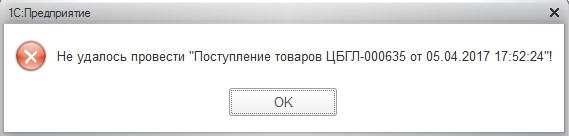
\includegraphics[width=0.8\textwidth]{28.jpg}
		\caption{Ошибка проведения.}
		\label{ris:28.jpg}
	\end{figure}
	И после закрытия этого сообщения показывается отчет по строкам документа, в которых имеется расхождение превышающее установленный порог с указанием цены в документе, цены плановой и суммы расхождения. Рис.~\ref{ris:29.jpg}
	\begin{figure}[H]
		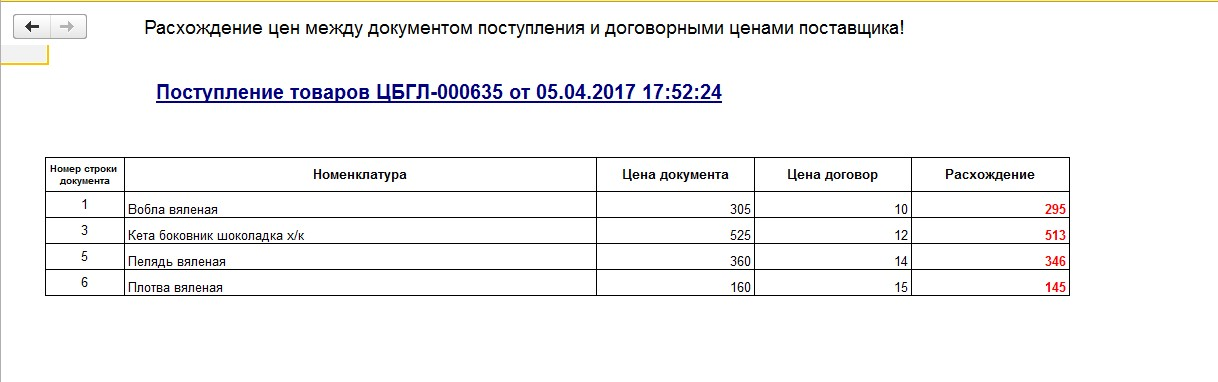
\includegraphics[width=0.8\textwidth]{29.jpg}
		\caption{Отчет по расхождениям в документе.}
		\label{ris:29.jpg}
	\end{figure}
	Одновременно на указанный ранее адрес электронной почты уходит письмо, в которое включен отчет об ошибке.
\end{itemize}
